\chapter{Monitoring}
\label{chap:monitoring}

Nu de gehele testomgeving geconfigureerd en werkende is, dient het hele gebeuren gemonitord worden. Dit is nodig om verschillende gegevens te verzamelen zodat er nadien kan worden overgegaan tot het evalueren van het allocatieschema in de proof-of-concept. In dit hoofdstuk wordt eerst dieper ingegaan op één specifieke tool, namelijk Rally~\cite{OpenStack2017b}, dat de deployment van OpenStack kan verifiëren. Vervolgens zal er een overzicht gegeven worden van de verschillende monitortechnieken waarna er ten slotte dieper wordt ingegaan op de gebruikte monitortechniek.

\section{Rally: evalueren schaalbaarheid OpenStack}
\label{sec:rally}

Rally~\cite{OpenStack2017b} is een benchmarking tool dat een OpenStack deployment kan automatiseren, de uitgerolde cloud kan verifiëren, benchmark testen kan uitvoeren en de cloud profileren. Het biedt daardoor een antwoord op de vraag hoe OpenStack werkt op grote schaal. Rally wordt gebruikt in drie high-level use cases die zeer interessant zijn om de deployment van OpenStack te evalueren. Een eerste use case is de mogelijkheid om een OpenStack omgeving te deployen, te testen en afhankelijk van de testresultaten OpenStack opnieuw te deployen met een andere configuratie tot de testen succesvol zijn. De tweede use case is bedoeld voor DevOps waarbij een bestaande cloud getest wordt met een simulatie van echte gebruikerswerklast waarna de resultaten worden weergegeven in allerhande grafieken. Een interessante eigenschap hierbij is dat SLA's gedefinieerd kunnen worden zodat hiermee rekening wordt gehouden tijdens het uitvoeren van de testen. De laatste use case is Rally CI/CD\footnote{\textit{Continuous Integration} en\textit{ Continuous Deployment}}, waarbij OpenStack wordt uitgerold op specifieke hardware met de laatste versie van een eigen geschreven tool. Hierop worden dan testen uitgevoerd die nadien gedeeld worden met de OpenStack community om zo OpenStack te verbeteren in de toekomst.

Rally maakt gebruik van 2 types invoerbestanden, namelijk een standaard JSON-bestand, of een YAML-bestand, een template-syntax gebaseerd op Jinja2\footnote{Een template engine geschreven in pure Python}. Elk invoerbestand bevat dan één of meerdere scenario's, al dan niet met meerdere configuraties per scenario. De configuratie van een scenario bevat steeds een lijst met argumenten (args) zoals de te gebruiken flavor, image, parameters, etc., de context die de gesimuleerde gebruikers representeert en een runner die bepaalt hoe de test wordt uitgevoerd. Optioneel kan er een nog een SLA, zoals bijvoorbeeld maximum aantal seconden per iteratie en de \textit{failure rate}, toegevoegd worden dat de eigenlijke succescriteria omschrijft.

Een voorbeeld om Rally beter te leren begrijpen maakt gebruik van een \textit{sample} invoerbestand en toont het verschil tussen een \textit{all-in-one} OpenStack deployment en een multi-node OpenStack deployment. Het invoerbestand ziet eruit als volgt:

\begin{code}
\begin{minted}[breaklines, fontsize=\footnotesize]{json}
{ % set flavor_name = flavor_name or "m1.tiny" %}
{  "NovaServers.boot_and_delete_server": [{
    "args": {
    "flavor": {
      "name": "{{flavor_name}}"
    },
    "image": {
      "name": "^cirros.*-disk$"
    },
    "force_delete": false
  },
  "runner": {
    "type": "constant",
    "times": 10,
    "concurrency": 2
  },
  "context": {
    "users": {
      "tenants": 3,
      "users_per_tenant": 2
      }}}, {
    "args": {
      "flavor": {
        "name": "{{flavor_name}}"
        },
      "image": {
        "name": "^cirros.*-disk$"
        },
      "auto_assign_nic": true
    },
    "runner": {
      "type": "constant",
      "times": 10,
      "concurrency": 2
    },
    "context": {
      "users": {
        "tenants": 3,
        "users_per_tenant": 2
      },
      "network": {
        "start_cidr": "10.2.0.0/24",
        "networks_per_tenant": 2
      }}}]}
\end{minted}
\caption{Rally test}
\end{code}

Dit invoerbestand stelt een scenario, NovaServers.boot\textunderscore and\textunderscore delete\textunderscore server, voor met twee configuraties. De eerste configuratie maakt gebruik van de flavor m1.tiny tenzij er een andere wordt meegegeven op de commandolijn, de standaard meegeleverde cirros image en de force\textunderscore delete option ingesteld op false. De runner-instelling bepaalt dat het proces 10 keer herhaald wordt waarbij er twee iteraties tegelijkertijd kunnen gebeuren (concurrency) en de context stelt de 6 gebruikers voor, verdeeld over 3 tenants. De tweede configuratie is grotendeels dezelfde als de eerste en bovendien wordt er een extra network-optie meegegeven.

Met bovenstaand invoerbestand kan de test worden uitgevoerd, eerst op een all-in-one omgeving met 1 node, vervolgens op de testomgeving zoals beschreven in Hoofdstuk~\ref{sec:environment}. De test uitvoeren gebeurt via volgend commando:

\begin{code}
\begin{minted}[breaklines]{bash}
$ rally task start `/opt/stack/rally/samples/tasks/scenarios/nova/
boot-and-delete.json`
\end{minted}
\end{code}

Na het uitvoeren van de test zijn de resultaten beschikbaar voor exporteren. Via volgend commando worden de resultaten geëxporteerd in een HTML-bestand:

\begin{code}
\begin{minted}[breaklines]{bash}
$ rally task report --out=report1.html
\end{minted}
\end{code}

Na het uitvoeren van de testen op beide omgevingen zijn er twee rapporten beschikbaar, één voor elke omgeving. De belangrijkste gegevens worden weergegeven in Figuur~\ref{fig:rally-test1} en Figuur~\ref{fig:rally-test2} en hierna besproken. De bovenste grafieken stellen de resultaten van de eerste configuratie voor, de onderste grafieken stellen de resultaten van de twee configuratie voor.

\begin{figure}
  \centering
  \captionsetup{justification=centering}
  \begin{subfigure}{\textwidth}
    \centering
    \centerline{
      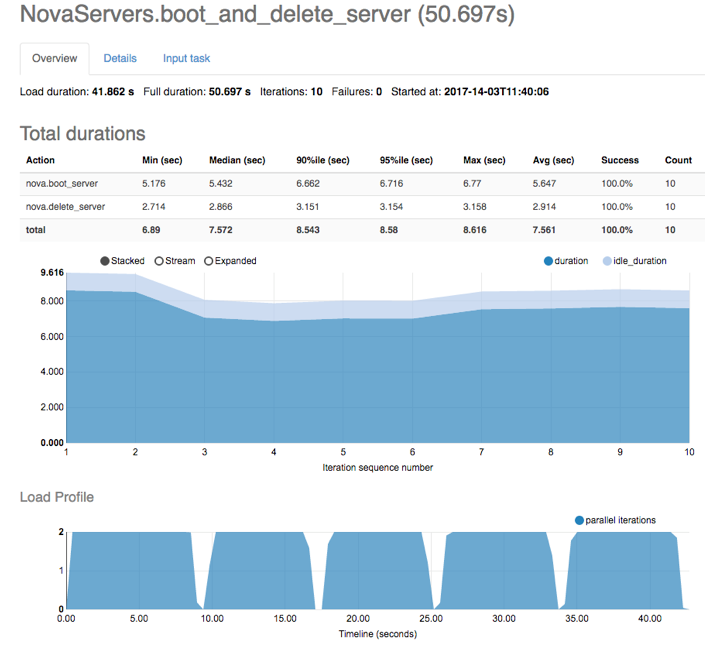
\includegraphics[scale=0.70]{Dia1}
    }
  \end{subfigure}
  \caption{Resultaat Rally-test: All-in-One Node}
  \label{fig:rally-test1}
\end{figure}

\begin{figure}
  \centering
  \captionsetup{justification=centering}
  \begin{subfigure}{\textwidth}
    \centering
    \centerline{
      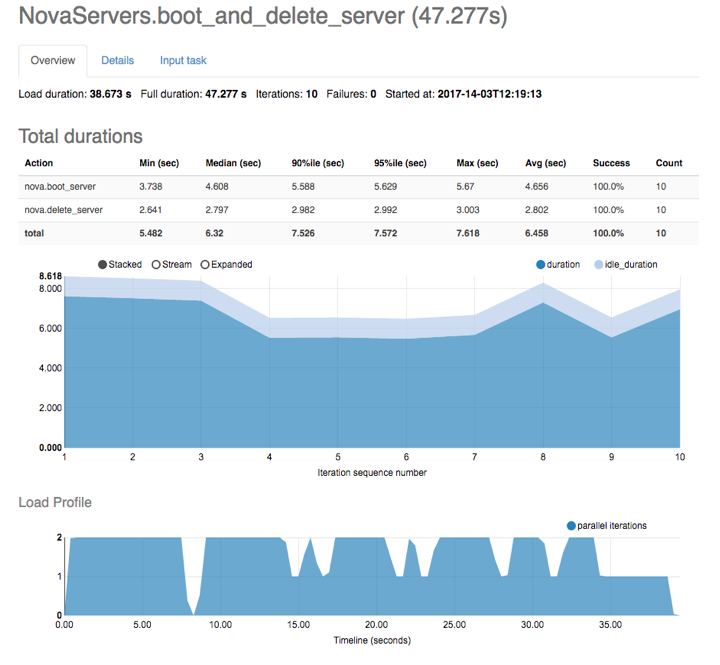
\includegraphics[scale=0.70]{Dia2}
    }
  \end{subfigure}
  \caption{Resultaat Rally-test: Testomgeving}
  \label{fig:rally-test2}
\end{figure}

Zoals te zien bovenaan in Figuur~\ref{fig:rally-test1} en Figuur~\ref{fig:rally-test2} is er een duidelijk verschil in de \textit{Load Profile} grafieken tussen beide opstellingen. Deze stellen het aantal parallelle iteraties voor in functie van de tijd en hieruit is duidelijk dat de testomgeving parallellisme beter ondersteund. Ook de tijd om een instantie te starten en te verwijderen is 12\% tot 20\% beter in de testomgeving dan in de all-in-one omgeving.
In de onderste grafieken is het meteen duidelijk dat de all-in-one opstelling faalt bij de laatste twee iteraties in tegenstelling tot de testomgeving. De tijd om een instantie te starten en te verwijderen is 16\% tot 27\% beter in de testomgeving dan in de all-in-one omgeving en het Load Profile is constanter in de testomgeving wat zorgt voor een betere betrouwbaarheid.

De testen uitgevoerd door Rally zijn nuttig om een nieuwe Nova-scheduler te evalueren op high-level niveau. Het ontwikkelen van een eigen test op een aangepaste Nova-scheduler biedt de mogelijkheid om deze nieuwe scheduler te testen met een vari"erende werklast waarbij de resultaten nadien eenvoudig worden omgezet in grafieken. Een belangrijk aspect is dat hiermee bekeken wordt of de nieuwe scheduler niet faalt om nieuwe instanties te creëren bij een stijgende werklast.

\section{Mogelijkheden om te monitoren}

Deze sectie geeft een overzicht weer van de verschillende mogelijkheden om een OpenStack-cloud te monitoren en data te verzamelen. Elke mogelijkheid zal tevens ook kort worden toegelicht met een eventueel voorbeeld.

\subsection{Nodejs-agent}
\label{sec:nodejs-agent}

Het monitoren van de drie hypervisors zal gebeuren met behulp van een zelf ontwikkelde Node.js-agent. Deze applicatie is een Node.js-applicatie die zal draaien op elk van de hypervisors. Met behulp van \textit{Express}, een \textit{npm package}, wordt er een node-server geïnitialseerd en gestart die vervolgens zal luisteren naar aanvragen op een vooraf ingestelde poort. Op dit ogenblik zijn volgende aanvragen geïmplementeerd:

\begin{itemize}
  \item \textit{/ping}: verwacht geen query, en geeft een 1 terug als resultaat (\textit{text/plain})
  \item \textit{/mongodb}: verwacht geen query, en geeft een JSON-string terug met het huidig resource-verbruik (\textit{application/json})
  \item \textit{/periodstats}: verwacht een query met 2 parameters, start en stop, waarbij beiden een tijdstip omschrijven met als vorm yyyy-dd-mmThh:mm:ss.xxxZ en geeft een JSON-string terug met het resource-verbruik tussen de twee meegegeven tijdstippen (\textit{application/json})
  \item \textit{/ceilometerstats}: verwacht een query met 2 parameters, start en stop, waarbij beiden een tijdstip omschrijven met als vorm yyyy-dd-mmThh:mm:ss.xxxZ en geeft een JSON-string terug met de metingen van Ceilometer tussen de twee meegegeven tijdstippen (\textit{application/json})
  \item \textit{/timestats}: verwacht een query met 2 parameters, start en stop, waarbij beiden een tijdstip omschrijven met als vorm yyyy-dd-mmThh:mm:ss.xxxZ en geeft een JSON-string terug met het resource-verbruik tussen de twee meegegeven tijdstippen alsook de metingen van ceilometer, beiden geordend volgens tijdstip (\textit{application/json})
\end{itemize}

De ping-aanvraag geeft eenvoudig weer of de agent op de hypervisor bereikbaar en geactiveerd is door een 1 terug te sturen naar de aanvrager. De mongodb aanvraag is belangrijk voor de correcte werking van de andere aanvragen. Indien de agent zo een aanvraag krijgt zal hij met behulp van het node-package \textit{os-utils} het CPU-verbruik en de hoeveelheid vrij geheugen bepalen. Vervolgens zal de agent met behulp van het node-package \textit{mysql} een connectie maken met de MySQL-databank op de OpenStack-controller, namelijk jerico-03, om de hoeveelheid actieve instanties op te vragen die op de hypervisor gehost zijn. Al deze resultaten samen met het huidige tijdstip worden dan bewaard in een mongoDB-databank welke actief is op jerico-01. Deze resultaten worden ook teruggezonden naar de aanvrager in JSON-formaat en kunnen nadien ook opgevraagd worden via de andere aanvragen (met uitzondering van de ping aanvraag).

Indien een aanvraag wordt gestuurd naar periodstats samen met twee parameters, een start- en eindtijdstip, zal de agent alle data van alle hypervisors tussen deze twee tijdstippen opvragen van de mongoDB op jerico-01. Een aanvraag naar ceilometerstats is gelijkaardig, enkel zal hier een aanvraag worden gestuurd naar de MongoDB op jerico-03 om zo alle statistieken die Ceilometer gemeten heeft binnen de meegegeven periode terug te geven aan de aanvrager. De timestats-aanvraag is een combinatie van de laatste twee, mits enkele aanpassingen. Zo wordt de data van ceilometer opnieuw opgevraagd van de MongoDB op jerico-03 en worden ook de instanties van de MySQL-databank op jerico-03 opgevraagd, beiden met het bijhorende tijdstip. Een combinatie van deze resultaten wordt nadien bezorgd aan de aanvrager.

\subsection{Grafana}

Grafana~\cite{Labs} is een van de meest bekende open-source software voor tijdsreeksanalyse. Het biedt een krachtige en elegante manier aan voor het creëren, ontdekken en delen van dashboards en data met een team of de hele wereld. Dankzij verschillende plugins is het mogelijk om variërende panelen, die onder andere grafieken bevatten, te configureren en te analyseren.

Ook een OpenStack-cloud kan met Grafana gemonitord en geanalyseerd worden indien aan bepaalde voorwaarden voldaan is. Zo moet OpenStack gebruikmaken van de Gnocchi-database waar Ceilometer zijn statistieken zal bewaren. Gnocchi~\cite{OpenStack2017d} is een projectnaam voor een TDBaaS (Time Series Database as a Service) project dat moet samenwerken met OpenStack Ceilometer. Het voordeel van deze benadering is dat vele metrieken, van de temperatuur tot het CPU-gebruik, worden bewaard per tijdstip en zo eenvoudig kunnen worden opgevraagd. Grafana kan dan met behulp van de Gnocchi-plugin\footnote{\url{https://grafana.com/plugins/sileht-gnocchi-datasource}} en de nodige configuratie een volledige OpenStack-cloud monitoren met een mogelijk resultaat zoals in Figuur~\ref{fig:grafana}.

\begin{figure}
  \centering
  \captionsetup{justification=centering}
  \begin{subfigure}{\textwidth}
    \centering
    \centerline{
      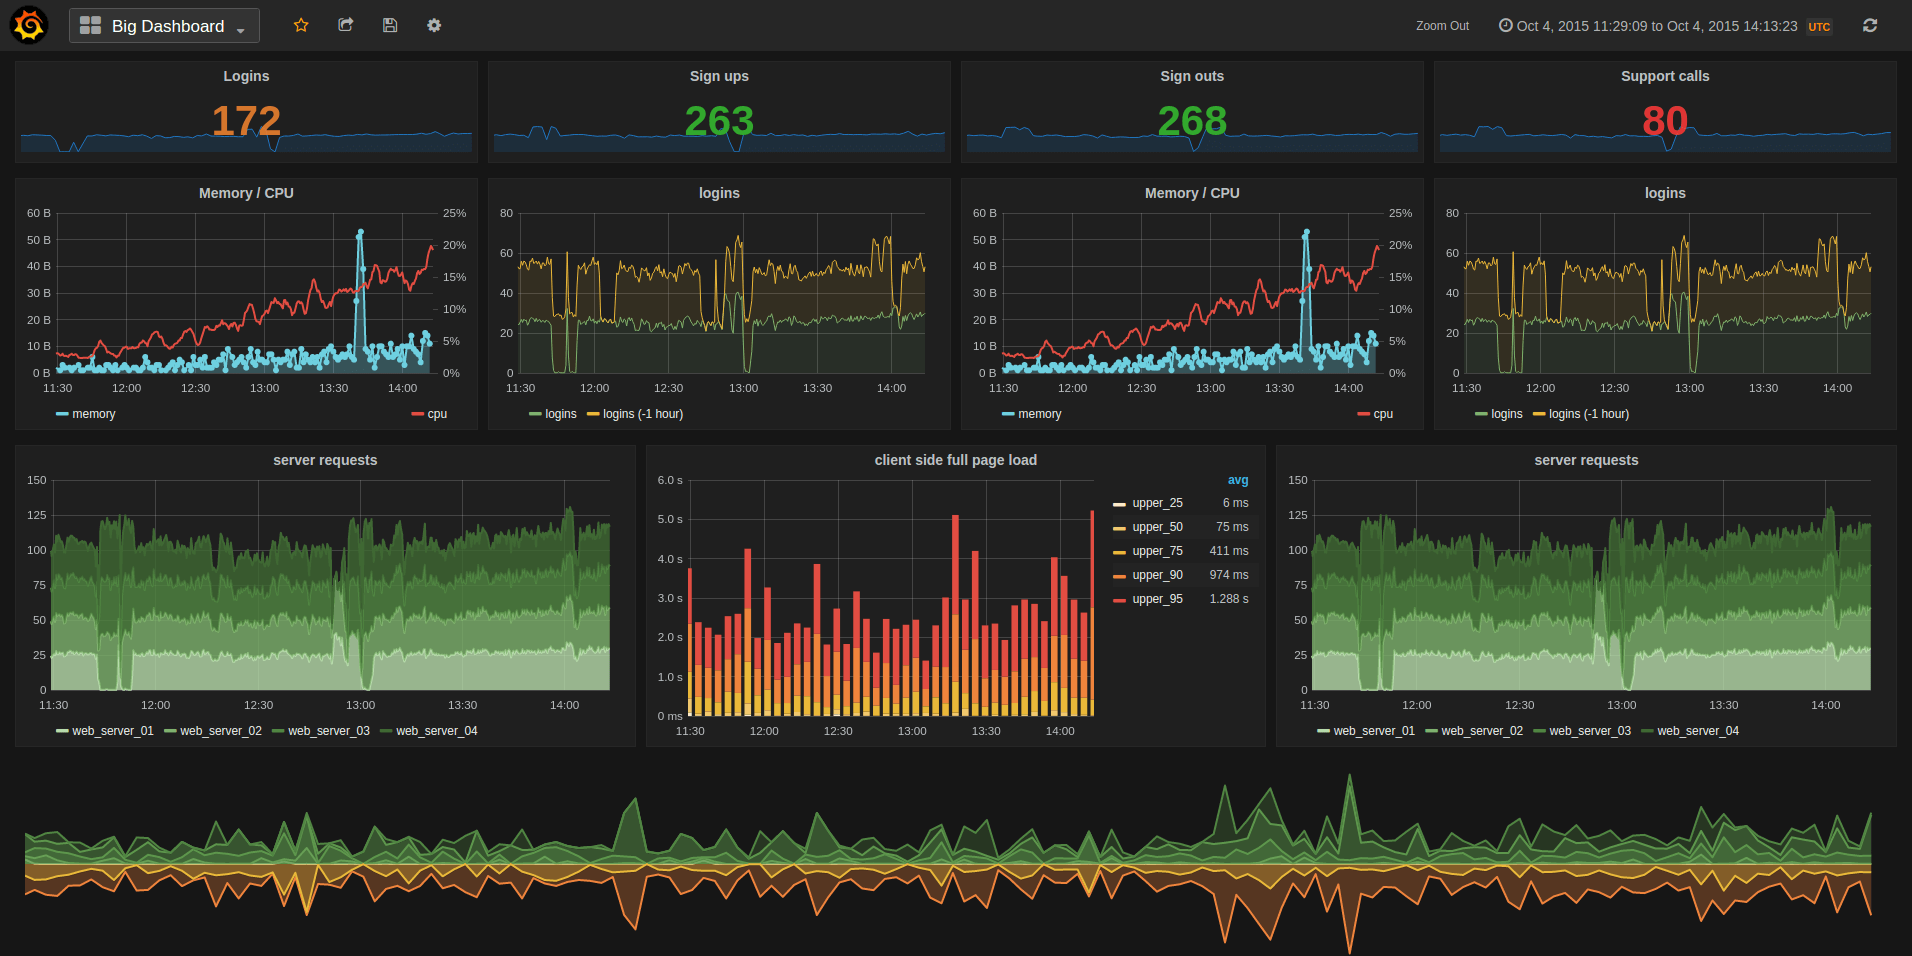
\includegraphics[scale=0.237]{dashboard_ex1}
    }
  \end{subfigure}
  \caption{Mock-up van een Grafana-dashboard}
  \label{fig:grafana}
\end{figure}

Het grootste voordeel van Grafana is dat het eenvoudig uitbreidbaar is naar andere cloud-structuren zonder al te veel wijzigingen. Daarnaast is het snel, performant en is er absolute vrijheid waar de Grafana-host zal draaien. De nadelen zijn echter de complexiteit om alles te configureren en het verplicht gebruik van Gnocchi in een OpenStack-cloud. Aangezien Gnocchi niet wordt gebruikt in de testomgeving (waar gebruik wordt gemaakt van MongoDB), biedt Grafana geen mogelijke manier om de evaluatie uit te voeren.

\subsection{Datadog}

Datadog~\cite{Datadog} is een softwarepakket in combinatie met een webapplicatie voor het monitoren van clouds. Dankzij meer dan 150 integraties van verschillende cloud-systemen zoals Amazon EC2, Kubernetes en ook OpenStack is het uitermate geschikt voor de monitoring van een cloud. Om Datadog te integreren met OpenStack moet de Datadog Agent geïnstalleerd worden op de hosts die dienst doen als hypervisor. Vervolgens kunnen er via een beveiligde omgeving op de website van Datadog online dashboards worden gecreëerd zodat er verschillende metrieken gemonitord worden. Een voorbeeld van zo'n dashboard is te zien in Figuur \ref{fig:datadog}.

\begin{figure}
  \centering
  \captionsetup{justification=centering}
  \begin{subfigure}{\textwidth}
    \centering
    \centerline{
      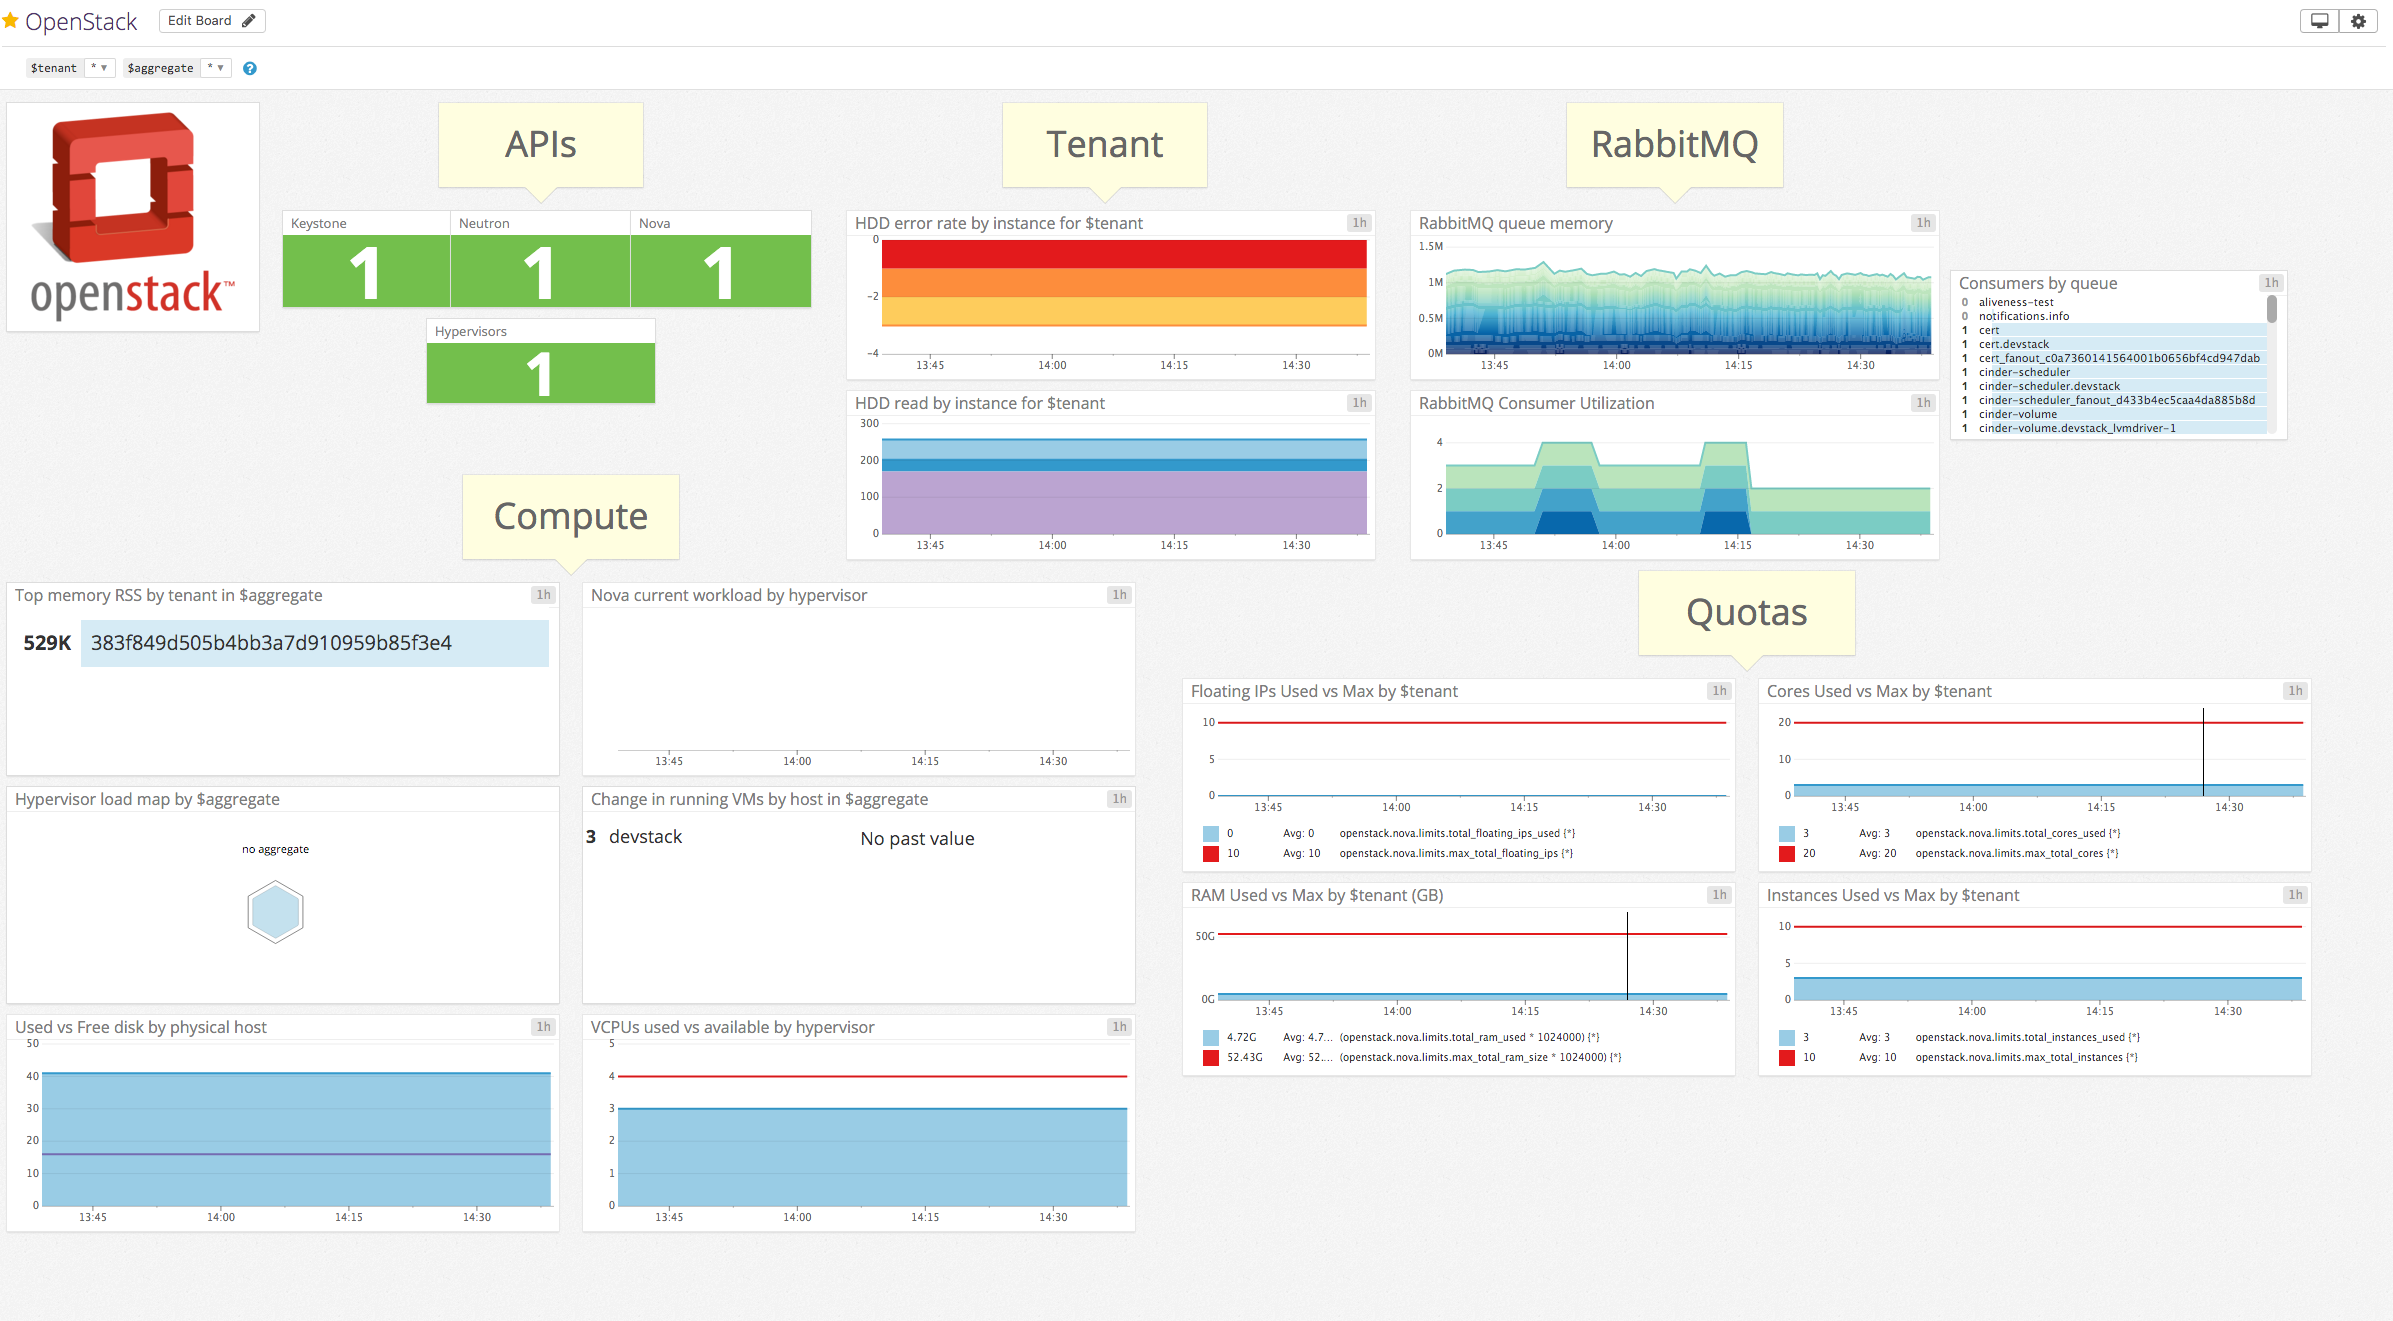
\includegraphics[scale=0.195]{datadog}
    }
  \end{subfigure}
  \caption{Mock-up van een Datadog-dashboard}
  \label{fig:datadog}
\end{figure}

Net zoals bij Grafana is het grote voordeel bij Datadog de overdraagbaarheid naar andere cloud-systemen. Daarnaast is het ook veel eenvoudiger in gebruik dankzij een eenvoudige installatie en configuratie. Datadog is beschikbaar als een gratis versie met een beperking van maximum 5 hosts waarbij enkel de standaard metrieken slechts 1 dag worden bewaard. Het grote nadeel is dat de prijs voor een beter pakket dat complexere metrieken en een langere bewaartijd biedt. Bijgevolg werd Datadog niet gekozen als optie om resource-allocatieschema's te evalueren.

\subsection{Overige mogelijkheden}

Verschillende overige mogelijkheden staan opgelijst op de monitoringpagina van OpenStack.\footnote{\url{https://wiki.openstack.org/wiki/Operations/Monitoring}} In deze lijst staan naast Rally en Datadog ook nog enkele interessante opties zoals Monasca~\cite{Openstack2017e}, een lopend OpenStack-project voor een open-source, schaalbaar, performant en fouttollerant \textit{monitoring-as-a-service} oplossing binnenin OpenStack. Andere mogelijkheden zijn bijvoorbeeld Graphite, Ganglia, Nagios, Stacktach, etc.

\section{Monitoring met Node.js en C3.js}
\label{sec:monitor_tool}

De uiteindelijke techniek om te monitoren maakt gebruik van de nodejs-agent in combinatie met een zelf ontwikkelde webapplicatie met c3.js~\cite{Tanaka2014} voor het weergeven van de grafieken. In deze sectie wordt dieper ingegaan op de nodejs-agent en de webapplicatie.

\subsection{Implementatie van de nodejs-agent}

Zoals beschreven in Sectie~\ref{sec:nodejs-agent} is de nodejs-agent een Node.js-applicatie die gebruikmaakt van verschillende node-packages. Deze applicatie is zo geschreven dat er eenvoudig nieuwe hosts kunnen worden toegevoegd of verwijderd. De code is beschikbaar via GitHub\footnote{\url{https://github.ugent.be/jfmoeyer/EvaluationRASOpenStack/tree/master/nodejs-agent}} en hier worden enkele stukken code kort toegelicht voorafgegaan door de vereisten.

Om de applicatie te kunnen starten zijn er enkele vereisten. Zo moet elke host waar de applicatie zal draaien voorzien zijn van Node.js en npm. Vervolgens moet er een MongoDB zijn die toegankelijk is voor alle hosts (eventueel met gebruikersnaam en wachtwoord). Deze databank bezit 1 tabel met de naam \textit{monitoring} en $n$ collecties waarbij $n$ staat voor het aantal hosts die gemonitord zullen worden. De databank waar Ceilometer de gegevens bewaard (in de testomgeving is dat de MongoDB op jerico-03) moet ook toegankelijk zijn voor externe verbindingen. Let wel op dat er geen authenticatie wordt ingesteld op deze databank want dit kan de werking van Ceilometer ernstig verstoren.

Een bestand dat steeds aanwezig is in een Node.js-applicatie is het package.json-bestand. Hier wordt meer informatie over de applicatie gegeven, welke commando's er uitgevoerd kunnen worden maar vooral welke afhankelijkheden (\textit{dependencies}) er nodig zijn om de geschreven code te kunnen uitvoeren. De belangrijkste afhankelijkheden hier zijn onder andere \textit{Express}, \textit{MongoDB}, \textit{Q}, etc.

Het bestand config.json bevat de nodige configuratie voor het uitvoeren van de applicatie. Hierin staan onder andere de verschillende hosts die gemonitord moeten worden, in welke tabellen de data wordt bewaard, op welke host de code wordt uitgevoerd, welke poort Express zal gebruiken, etc. In het geval van de testomgeving moest dankzij dit configuratiebestand enkel de variabele \textit{current\textunderscore host} worden aangepast per verschillende host zodat de applicatie weet op welke host hij actief is.

Systeminfo.js bevat de drie verschillende methodes die metrieken zal meten, bewaren en teruggeven. De eerste methode \textit{updateMongoDB(callback)} zal de drie metrieken, CPU-gebruik, vrij geheugen en aantal actieve instanties van de huidige host opvragen, bewaren in de MongoDB en deze ook teruggeven. De code van deze functie ziet er als volgt uit:

\begin{code}
\begin{minted}[breaklines]{javascript}
method.updateMongoDB = (callback) => {
  os.cpuUsage((cpu_usage) => {
    var free_mem = os.freemem();
    connection.query("SELECT host, count(*) from instances where power_state = 1 and host like '" + HOST_NAME + "' group by host", (error, result, fields) => {
      if (result[0]) {
        var instances = result[0]['count(*)'];
      } else {
        var instances = 0;
      }
      MongoClient.connect(url_monitoring, (err, db) => {
        assert.equal(null, err);
        insertDocument(db, cpu_usage, free_mem, instances, () => {
          db.close();
          callback({
            "cpu_usage": cpu_usage,
            "free_mem": free_mem,
            "instances": instances,
            "timestamp": new Date()
  });});});});});
}
\end{minted}
\caption{nodejs-agent: updateMongoDB-functie}
\end{code}

Als eerste wordt het CPU-gebruik berekend met behulp van de node-package \textit{os-utils}. Vervolgens wordt met hetzelfde pakket de hoeveelheid vrij geheugen opgevraagd. Daarna maakt de applicatie connectie met de MySQL-host om de hoeveelheid actieve instanties op de host te bepalen. Dit alles wordt tenslotte in de MongoDB bewaard en teruggegeven als JSON-object.

De tweede methode \textit{getPeriodStatsScale(start, end, callback)} zal de statistieken tussen een bepaalde periode (tussen start en stop) downloaden vanaf de MongoDB. De gebruikte code ziet er als volgt uit:

\begin{code}
\begin{minted}[breaklines]{javascript}
method.getPeriodStatsScale = (start, end, callback) => {
  var promises = [];
  MongoClient.connect(url_monitoring, (err, db) => {
    assert.equal(null, err);
    var complete_result = {};
    for (var node of appConfig.nodes) {
      complete_result[node.server_name + " CPU"] = [];
      complete_result[node.server_name + " Memory"] = [];
      complete_result[node.server_name + " Instances"] = [];
      var cursor = db.collection(node.mongo_table_name).find({ "timestamp": { $gt: new Date(start), $lt: new Date(end) } });
      var promise = new Promise((resolve, reject) => {
        var node_name = node.server_name;
        cursor.each((err, doc) => {
          if (err) {
            reject("Something went wrong with node " + node_name);
          }
          if (doc != null) {
            complete_result[node_name + " CPU"].push(doc.cpu_usage);
            complete_result[node_name + " Memory"].push(doc.free_mem);
            complete_result[node_name + " Instances"].push(doc.instances);
          } else {
            resolve(node_name + " is inserted!");
      }});});
      promises.push(promise);
    }
    Q.all(promises).then(() => {
      db.close();
      callback(complete_result);
    }).fail(console.error);
  });
}
\end{minted}
\caption{nodejs-agent: getPeriodStatsScale-functie}
\end{code}

De belangrijkste functionaliteit van deze functie is het gebruik van Promises binnen JavaScript. Dit laat namelijk toe dat indien er een connectie is met de MongoDB, elke node uit het conf.json-bestand overlopen wordt en dit bepaalde methodes zal uitvoeren (zoals alle metrieken opvragen). Vervolgens zal dankzij het node-package \textit{Q} gewacht worden totdat alle Promises voltooid zijn waarna het verkregen resultaat kan worden teruggegeven.

De laatste methode om metrieken op te vragen is \textit{getCeilometerAndInstancesTimeScale(start, stop, callback)}. Deze dient om de werklast, gemeten door Ceilometer, op te vragen samen met het aantal instanties per host. De gebruikte code ziet er uit als volgt:

\begin{code}
\begin{minted}[breaklines]{javascript}
method.getCeilometerAndInstancesTimeScale = (start, stop, callback) => {
  MongoClient.connect(url_ceilometer, (err, db) => {
    assert.equal(null, err);
    var cursor = db.collection("meter").find({ timestamp: { $gt: new Date(start), $lt: new Date(stop) }, counter_name: appConfig.scale_app.counter_name, "resource_metadata.display_name": appConfig.scale_app.scale_group_name, "resource_metadata.status": "active" });
    var result = {};
    var complete_result = {};
    var promises = [];
    cursor.each((err, doc) => {
      if (doc != null) {
        result[doc.timestamp] = doc.counter_volume;
      } else {
        db.close();
          MongoClient.connect(url_monitoring, (err, db) => {
            assert.equal(null, err);
            for (var node of appConfig.nodes) {
              complete_result[node.server_name] = {};
              var cursor = db.collection(node.mongo_table_name).find({ "timestamp": { $gt: new Date(start), $lt: new Date(stop) } });
              var promise = new Promise((resolve, reject) => {
                var node_name = node.server_name;
                cursor.each((err, doc) => {
                  if (err) {
                    reject("Something went wrong with node " + node_name)
                  }
                  if (doc != null) {
                    complete_result[node_name][doc.timestamp] = doc.instances;
                  } else {
                    resolve(node_name + " is inserted!");
              }});});
            promises.push(promise);
            }
          Q.all(promises).then(() => {
            db.close();
            callback([result, complete_result]);
          }).fail(console.error);
  });}});});
}
\end{minted}
\caption{nodejs-agent: getCeilometerAndInstancesTimeScale-functie}
\end{code}

Hier wordt eveneens gebruikgemaakt van Promises om alle hosts in het configuratiebestand te overlopen. Eerst worden de gegevens van de ceilometer-databank opgevraagd en nadien de metrieken van elke host. Op het einde van de code wordt er gewacht tot alle Promises zijn voltooid alvorens het resultaat wordt teruggegeven aan de callback-functie.

Het laatste bestand in deze applicatie heet \textit{rpicluster.agent.js}. Dit is het kloppend hart van de applicatie doordat deze de aanvragen vanuit de buitenwereld zal verwerken en uitvoeren. Met behulp van het Express-package van Node wordt er een router geïnitialiseerd, geconfigureerd en per aanvraag, zoals vermeld in Sectie~\ref{sec:nodejs-agent}, een functie geïmplementeerd. Een voorbeeld van zulke functie ziet er uit als volgt:

\begin{code}
\begin{minted}[breaklines]{javascript}
router.get("/timestats", function(req, res) {
  res.writeHead(200, { 'Content-Type': 'application/json'});
  var url_parts = url.parse(req.url, true);
  var query = url_parts.query;
  new Systeminfo().getCeilometerAndInstancesTimeScale(query.start, query.stop, (result) => {
    res.end(JSON.stringify(result));
  });
});
\end{minted}
\caption{nodejs-agent: nodejs-agent: implementatie van een aanvraag}
\end{code}

Vooraleer deze code tot stand is gekomen, werd er eerst gebruik gemaakt van asynchrone en hard-coded aanvragen die moeilijk uit te breiden waren naar meer of minder hosts. Dankzij de overschakeling naar het gebruik van Promises en het conf.json-bestand, zijn er twee voordelen. Er kunnen eenvoudig meerdere hosts worden toegevoegd of verwijderd (de databank die alles bewaard kan zelfs extern zijn) en dankzij het gebruik van de Promises is de code performanter omdat deze stukken code ``gelijktijdig'' uitgevoerd worden.

Om de nodejs-agent te starten zijn er slechts twee commando's nodig, één om de nodige afhankelijkheden te installeren en één om de applicatie te starten. De twee commando's, waarbij de \& in het laatste commando ervoor zorgt dat de applicatie in de achtergrond wordt uitgevoerd, zijn de volgende:

\begin{code}
\caption{Starten van de nodjs-agent}
\begin{minted}[breaklines]{bash}
$ sudo npm install
$ sudo npm start &
\end{minted}
\end{code}

\subsection{Implementatie van de webapplicatie}

De webapplicatie bestaat uit twee pagina's, één voor live-monitoring en één voor het opvragen van gegevens die gemeten zijn tijdens een bepaalde periode (op voorwaarde dat er tijdens die periode live-monitoring is gebeurd). Ze werkt nauw samen met de nodejs-agent voor het opvragen van gegevens en het aansturen van de databank. Ook in de webapplicatie werd gebruikgemaakt van een configuratiebestand zodat er eenvoudig meerdere hosts kunnen worden toegevoegd of verwijderd. De code is beschikbaar via GitHub\footnote{\url{https://github.ugent.be/jfmoeyer/EvaluationRASOpenStack/tree/master/webapp}} en maakt gebruik van c3.js~\cite{Tanaka2014} voor het visualiseren van de grafieken. Ook hier worden Promises gebruikt voor zowel betere performantie als schaalbaarheid. Aangezien de code zeer gelijkaardig is aan die van de nodejs-agent wordt deze hier ook niet verder besproken.

De live-monitoring pagina wordt weergegeven in Figuur~\ref{fig:webapp1} en Figuur~\ref{fig:webapp2} en de functionaliteiten worden hier kort besproken. De drie grafieken in deelfiguur (a) geven respectievelijk het CPU-gebruik, de hoeveelheid vrij geheugen en het aantal actieve instanties weer per host. Indien de gebruiker de grafieken wenst te verbergen tijdens een sessie, kan hij deze uitschakelen en zal een spinner aangeven of het monitoren bezig is of niet wat te zien is in deelfiguur (b). Bij een sessie zal er standaard elke 2 seconden (2000 ms) een aanvraag worden gestuurd naar de nodejs-agent voor het bewaren en teruggeven van de metrieken op dat moment (de /mongodb aanvraag van de nodejs-agent). Het interval kan aangepast worden naar belangen van de gebruiker. Vooraleer het monitoren kan gestart worden, is er een controle of de te monitoren hosts wel beschikbaar zijn. Dit gebeurt via een ping-aanvraag naar alle hosts en pas wanneer alle hosts antwoord geven, kan er gemonitord worden.

\begin{figure}
\centering
\subcaptionbox{Live monitoring - grafieken zichtbaar \label{fig:webapp1}}{%
  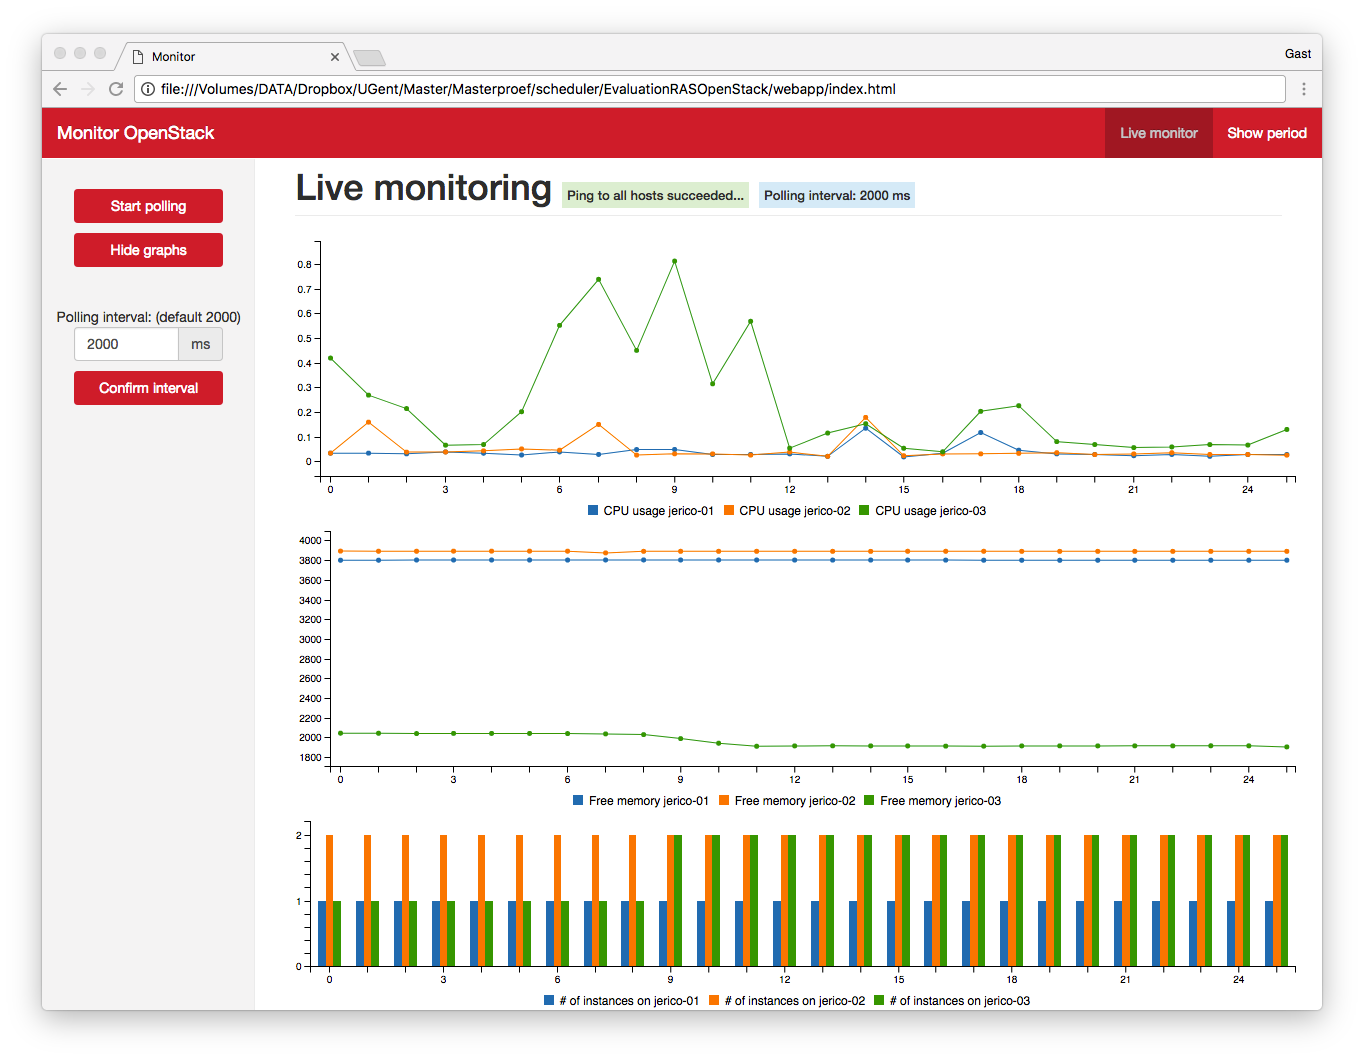
\includegraphics[width=0.65\textwidth]{webapp_img1}%
}\par\medskip
\subcaptionbox{Live monitoring - grafieken verborgen \label{fig:webapp2}}{%
  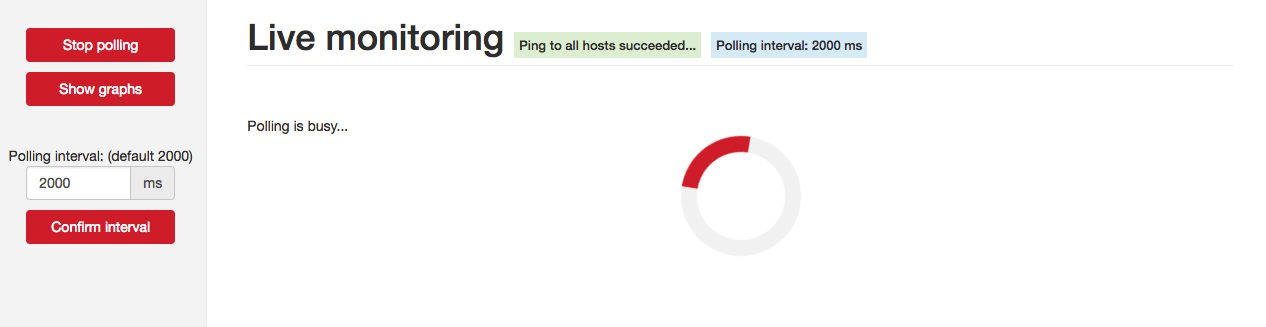
\includegraphics[width=0.65\textwidth]{webapp_img2}%
}\par\medskip
\subcaptionbox{Overzicht van een periode \label{fig:webapp3}}{%
  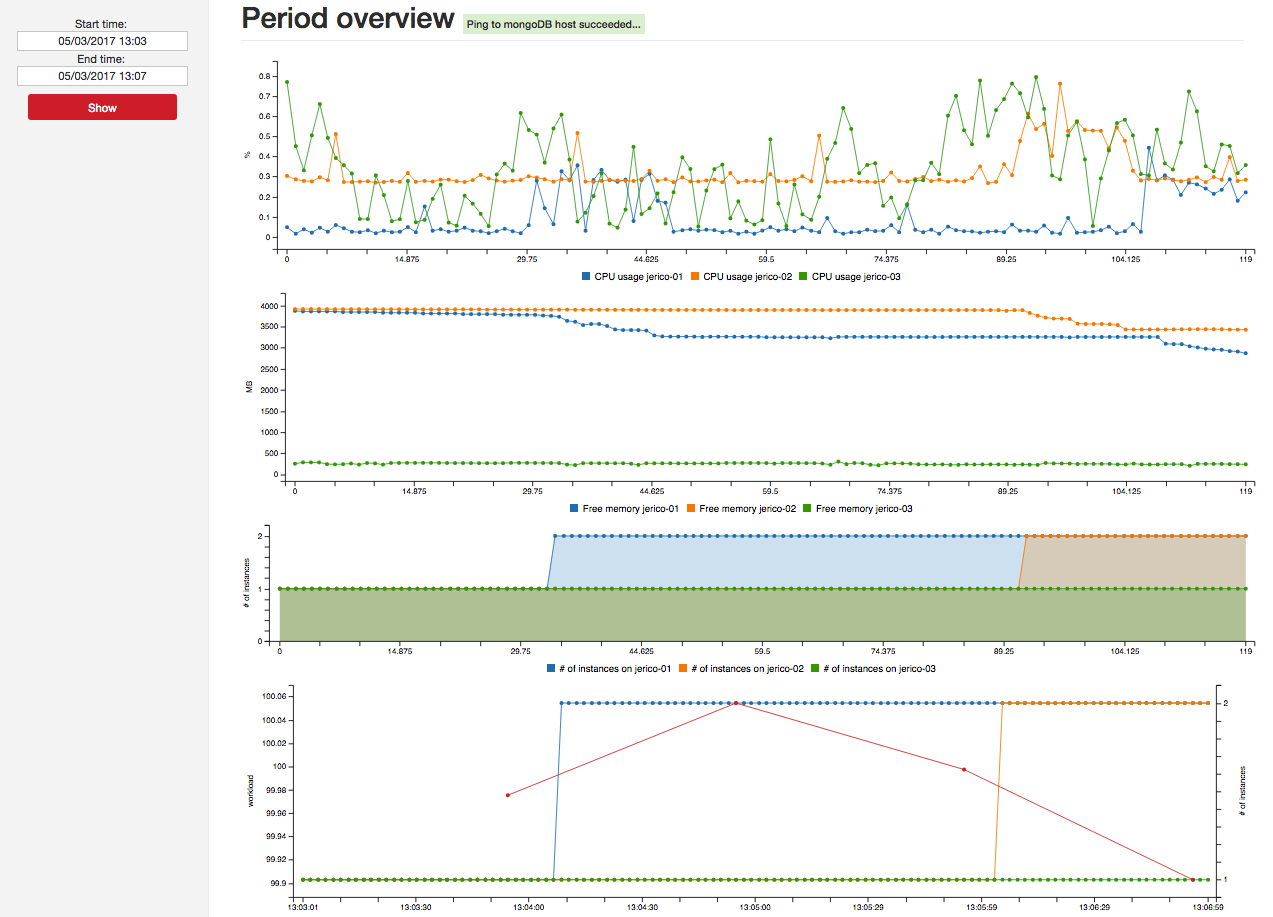
\includegraphics[width=0.65\textwidth]{webapp_img3}%
}
\caption{Webapplicatie}
\label{fig:webapp}
\end{figure}

De periode-pagina wordt weergegeven in Figuur~\ref{fig:webapp3} en is zeer gelijkaardig aan de live-monitor pagina. Hier wordt wel een extra grafiek weergegeven, die het aantal instanties per host combineert met de gemeten statistieken van Ceilometer. Onmiddellijk na het laden van de pagina wordt er gecontroleerd of de host die de databank bevat bereikbaar is. Enkel indien deze bereikbaar is kan er een periode worden ingevoerd en zal deze gevisualiseerd worden in de 4 grafieken.
